\documentclass[10pt]{article}
\usepackage[utf8]{inputenc}
\usepackage[swedish, english]{babel}
\usepackage[margin=2cm]{geometry}
\usepackage[utf8]{inputenc}
\selectlanguage{swedish}
\usepackage{graphicx}
\graphicspath{ {images/} }


\title{Kravspecifikation}

\author{
    Joel Almqvist\\
    \texttt{joeal360@student.liu.se}
    \and
    Björn Detterfelt\\
    \texttt{bjode786@student.liu.se}
    \and
    Tim Håkansson\\
    \texttt{timha404@student.liu.se}
    \and
    David Kjellström\\
    \texttt{davkj168@student.liu.se}
    \and
    Axel Löjdquist\\
    \texttt{axelo225@student.liu.se}
    \and
    Joel Oskarsson\\
    \texttt{joeos014@student.liu.se}
    \and
    Lieth Wahid\\
    \texttt{liewa893@student.liu.se}
    \and
    Alexander Wilkens\\
    \texttt{alewi684@student.liu.se}
}

\begin{document}

\maketitle
\pagebreak
\tableofcontents
\pagebreak
\section{Inledning}
	I detta kapitel definieras och introduceras kontexten för projektet som ska utföras.

	\subsection{Definitioner}
		\begin{itemize}
		\item UI applikationen -- Applikationen som kör själva spelet.
		\item Kontroll applikationen -- Applikationen som körs på en mobil eller surfplatta som styr spelet.
		\item HotJoin -- möjligheten att hoppa in i ett pågående spel
		\item Standard nätverksförhållande - Stabilt WiFi-LAN kopplad till en router med stabil ethernet uppkoppling.
		\item Sensor -- En sensor som sitter på kontrollern som inte är en touch-skärm (t.ex. en accelerometer)
		\end{itemize}	

	\subsection{Parter}
	Kunden till projektet är Cybercom Sweden. Projektet utförs av projektgruppens medlemmar.
	
	\subsection{Syfte \& mål}
		Syftet med projektet är att skapa en prototyp för att demonstrera Cybercoms IoT backend. För att kunna uppnå detta, ska ett realtidsmultiplayerspel skapas. Syftet för projektgruppens är att genomföra ett kandidatarbete enligt kursen TDDD96 -- Kandidatprojekt i programvaruutveckling mål.
	
	\subsection{Användning}
		För att kunna använda produkten måste två olika applikationer köras på minst två olika enheter. En mobil eller surfplatta ska användas som kontroll för att styra spelet och kommer att köra kontroll applikationen. Utöver detta ska en dator vara uppkopplad till en skärm. Datorn ska köra själva spelet och kommer att köra UI applikationen.  
	
	\subsection{Bakgrundsinformation}
		Projektgruppen har tidigare läst en kurs om programutvecklingsmetodik och vill omsätta denna kunskap i praktiken. 
		
\pagebreak
\section{Översikt av Systemet}
	Detta kapitel ger en överskådlig blick av systemet.

	\subsection{Grov beskrivning av produkten}
	Produkten ska vara ett realtidsmultiplayerspel. Spelet är uppdelat i två olika komponenter, en UI-del och en kontroller del. UI-delen är tänkt att agera som skärm för spelet och kan liknas med en konsol för ett TV-spel. På denna del kommer att själva spelet köras och vara uppkopplad till en skärm där spelet visas. En kontroller kommer vara antingen en mobil eller surfplatta och kan liknas med spelkontrollerna till konsolen. Enhetens sensorer används för att spelaren ska kunna styra spelet. Kommunikationen mellan UI-delen och kontroller-delen kommer att ske genom Cybercoms backend, se figur 1. Att kommunikationen går genom Cybercoms backend är vital eftersom huvudsyftet med projektet är att demonstrera Cybercoms IoT backend.  Både kontroller- och UI-delen kommer att utvecklas som progressiva webbappar. 
	
	\begin{figure}[h]
		\centering
		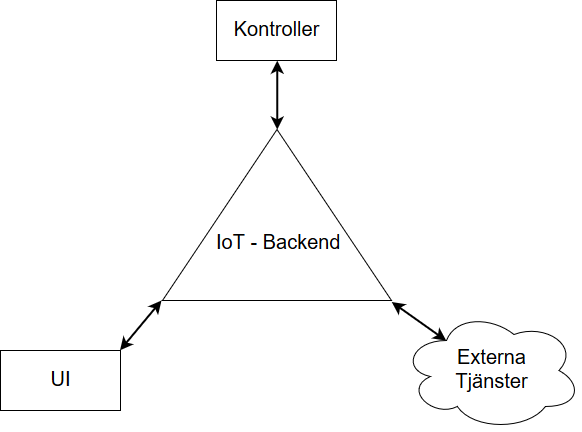
\includegraphics[scale=0.4]{backend}
		\caption{Kommunikation mellan Cybercoms backend och komponenterna i systemet}
		\label{fig:backend}
	\end{figure}
	
	
	\subsection{Beroenden av andra system}
	Produkten är beroende av Cybercoms backend då all kommunikation måste gå genom denna. Produkten är även beroende av en enhet som har tillgång till version 64 av Chrome. Produkten kräver även en enhet som kan köra UI-delen av systemet.

\pagebreak
\section{Krav}
	Detta avsnitt listar alla krav som sätts på produkten. Krav med prioritet 1 förväntas vara avklarade vid projektetsslut. Krav med prioritet 2 ska arbetas mot då alla krav med prioritet 1 är avklarade.
	\subsection{Funktionella Krav}
	Detta avsnitt listar de funktionella kraven på produkten.	
	
	\begin{tabular}{| p{2cm} | p{8cm} | p{2cm}|}
		\hline
		
		\textbf{Krav nr.} & \textbf{Beskrivning} &\textbf{Prioritet} \\ \hline
		Krav 1 & En mobil eller surfplatta ska användas som spelkontroll för spelet. & 1 \\ \hline
		Krav 2 & UI applikationen ska stödja ett minimum av 2 antal spelare & 1 \\ \hline
		Krav 3 & Kontroll applikationen ska ha ett grafiskt gränssnitt   & 1 \\ \hline
		Krav 4 & UI applikationen ska kunna köras på en enhet som har Chrome & 1 \\ \hline
		Krav 5 & Kontroll applikationen ska kunna köras på en enhet som har Chrome & 1 \\ \hline
		Krav 6 & UI applikationen ska endast kommunicera med Cybercoms backend & 1 \\ \hline
		Krav 7 & UI applikationen ska stödja version 64 av Chrome & 1 \\ \hline
		Krav 8 & Kontroll applikationen ska stödja version 64 av Chrome & 1 \\ \hline
		Krav 9 & En användare ska kunna gå in i en spelinstans & 1 \\ \hline
		Krav 10 & UI applikationen ska stödja hotjoinfunktionalitet & 1 \\ \hline
		Krav 11 & Flera instanser av spelet ska kunna köras samtidigt & 1 \\ \hline
		Krav 12 & Kontroll applikationen ska stödja styrning med tagentbord och mus & 2 \\ \hline
		Krav 13 & UI applikationen ska visa en unik kod för sin spelinstans & 2 \\ \hline
		Krav 14 & En spelinstans spelare ska kunna rösta på vilket spel som ska spelas & 1 \\ \hline
		Krav 15 & UI applikationen ska kunna starta en spelinstans & 1 \\ \hline
		Krav 16 & UI applikationen ska kunna avsluta en spelinstans & 1 \\ \hline
		Krav 17 & Kontroll applikationen ska kommunicera med Cybercoms backend & 1 \\ \hline
		Krav 18 & UI applikationen ska kommunicera med Cybercoms backend & 1\\ \hline
		Krav 19 & Kontroll applikationen ska kunna ansluta sig till en spelinstans genom att ange en ID-kod & 2 \\ \hline
		Krav 20 & En unik slumpmässig ID-kod ska kunna genereras för en spelinstans & 1 \\ \hline
		Krav 21 & UI applikationen ska kunna välja sin egna ID-kod för spelinstansen den kör & 2 \\ \hline
		
		
		
	\end{tabular}
	
	\subsection{Designkrav}
	Detta avsnitt listar kraven på utvecklingsprocessen
	
	\begin{tabular}{| p{2cm} | p{8cm} | p{2cm}|}
		\hline
		\textbf{Krav nr.} & \textbf{Beskrivning} & \textbf{Prioritet} \\ \hline
		
		Krav 22 & UI applikationen ska skrivas i Javascript ES2015+ & 1 \\ \hline
		Krav 23 & Kontroll applikationen ska skrivas i Javascript ES2015+ & 1 \\ \hline
		Krav 24 & UI applikationen ska utvecklas som en PWA & 1 \\ \hline
		Krav 25 & Kontroll applikationen ska utvecklas som en PWA & 1 \\ \hline
		Krav 26 & All kod som skrivs ska följa en dokumentationsstandard & 1 \\ \hline
		Krav 27 & UI applikationen ska licensieras under MITs opensource licens & 1 \\ \hline
		Krav 28 & Kontroll applikationen ska licensieras under MITs opensource licens & 1 \\ \hline
	\end{tabular}

	\subsection{Kvalitetskrav}
	Detta avsnitt listar krav på kvalitén hos den slutgilitga produkten.
	
		\begin{tabular}{|p{2cm}|p{8cm}|p{2cm}|}
		\hline
		\textbf{Krav nr.} & \textbf{Beskrivning} & \textbf{Prioritet} \\ \hline
		Krav 29 & UI applikationen ska kunna köras i 4 timmar utan avbrott & 1 \\ \hline
		Krav 30 & Arkitekturen för systemet ska vara designat så att det är möjligt att vidareutveckla projektet & 1 \\ \hline
		Krav 31 & Tiden att ansluta sig till en spelsession får inte överskrida 10 sekunder under standard nätverksförhållanden & 1 \\ \hline
		Krav 32 & & \\ \hline
		
	\end{tabular}

\end{document}